\documentclass[12pt,a4paper]{article}
\usepackage[ngerman]{babel}
\usepackage[utf8]{inputenc}
\usepackage[unicode=true,bookmarks=false,bookmarksopen=true]{hyperref}

\usepackage{xcolor}
\usepackage{graphicx}
\usepackage{tikz}

\usepackage{listings}

\def\checkmark{\tikz\fill[scale=0.4](0,.35) -- (.25,0) -- (1,.7) -- (.25,.15) -- cycle;}

\definecolor{pGreen}{rgb}{0.44, 0.71, 0}
\definecolor{nRed}{rgb}{0.74, 0, 0}

\title{ORES Custom Documentation VII}
%\author{Tom Gülenman}
\date{}
\begin{document}
\maketitle
\textit{Disclaimer: No guarantee for the correctness of information / explanations / sources is given.}\\
%
%
%
\section*{Goals}
\begin{enumerate}
\item Look further into visualisation possibilities for Use Case 1
\end{enumerate}
\section{Data Visualisations}
\underline{Use Case 1}: maximum recall @ precision $>=0.9$\\
%
\subsection{Quick brainstorming}
\begin{itemize}
\item Maybe we should not focus on constructing sdomething that works for Use Case 1, but already look for solutions that will help with every query.
\item The common factor are the confusion matrix values: TP, FP, TN, FN and still the best visualisation to me is the Google Discrimination Threshold one (\href{https://research.google.com/bigpicture/attacking-discrimination-in-ml/}{Link}).
\item I feel like constructing something like that and then showing pie charts or something similar to put the focus on the metrics of the query would be optimal, even though we don't need to be able to move the threshold. The threshold doesn't have to be the center of attention for a visualisation like that. It can just be put where it belongs automatically, based on the other metrics, to give a better understanding of where the negatives end and the positives start. 
\end{itemize}
%
\subsection{Concrete suggestions}
\begin{itemize}
\item Example of how the process could look like ...?:
\begin{description}
\item 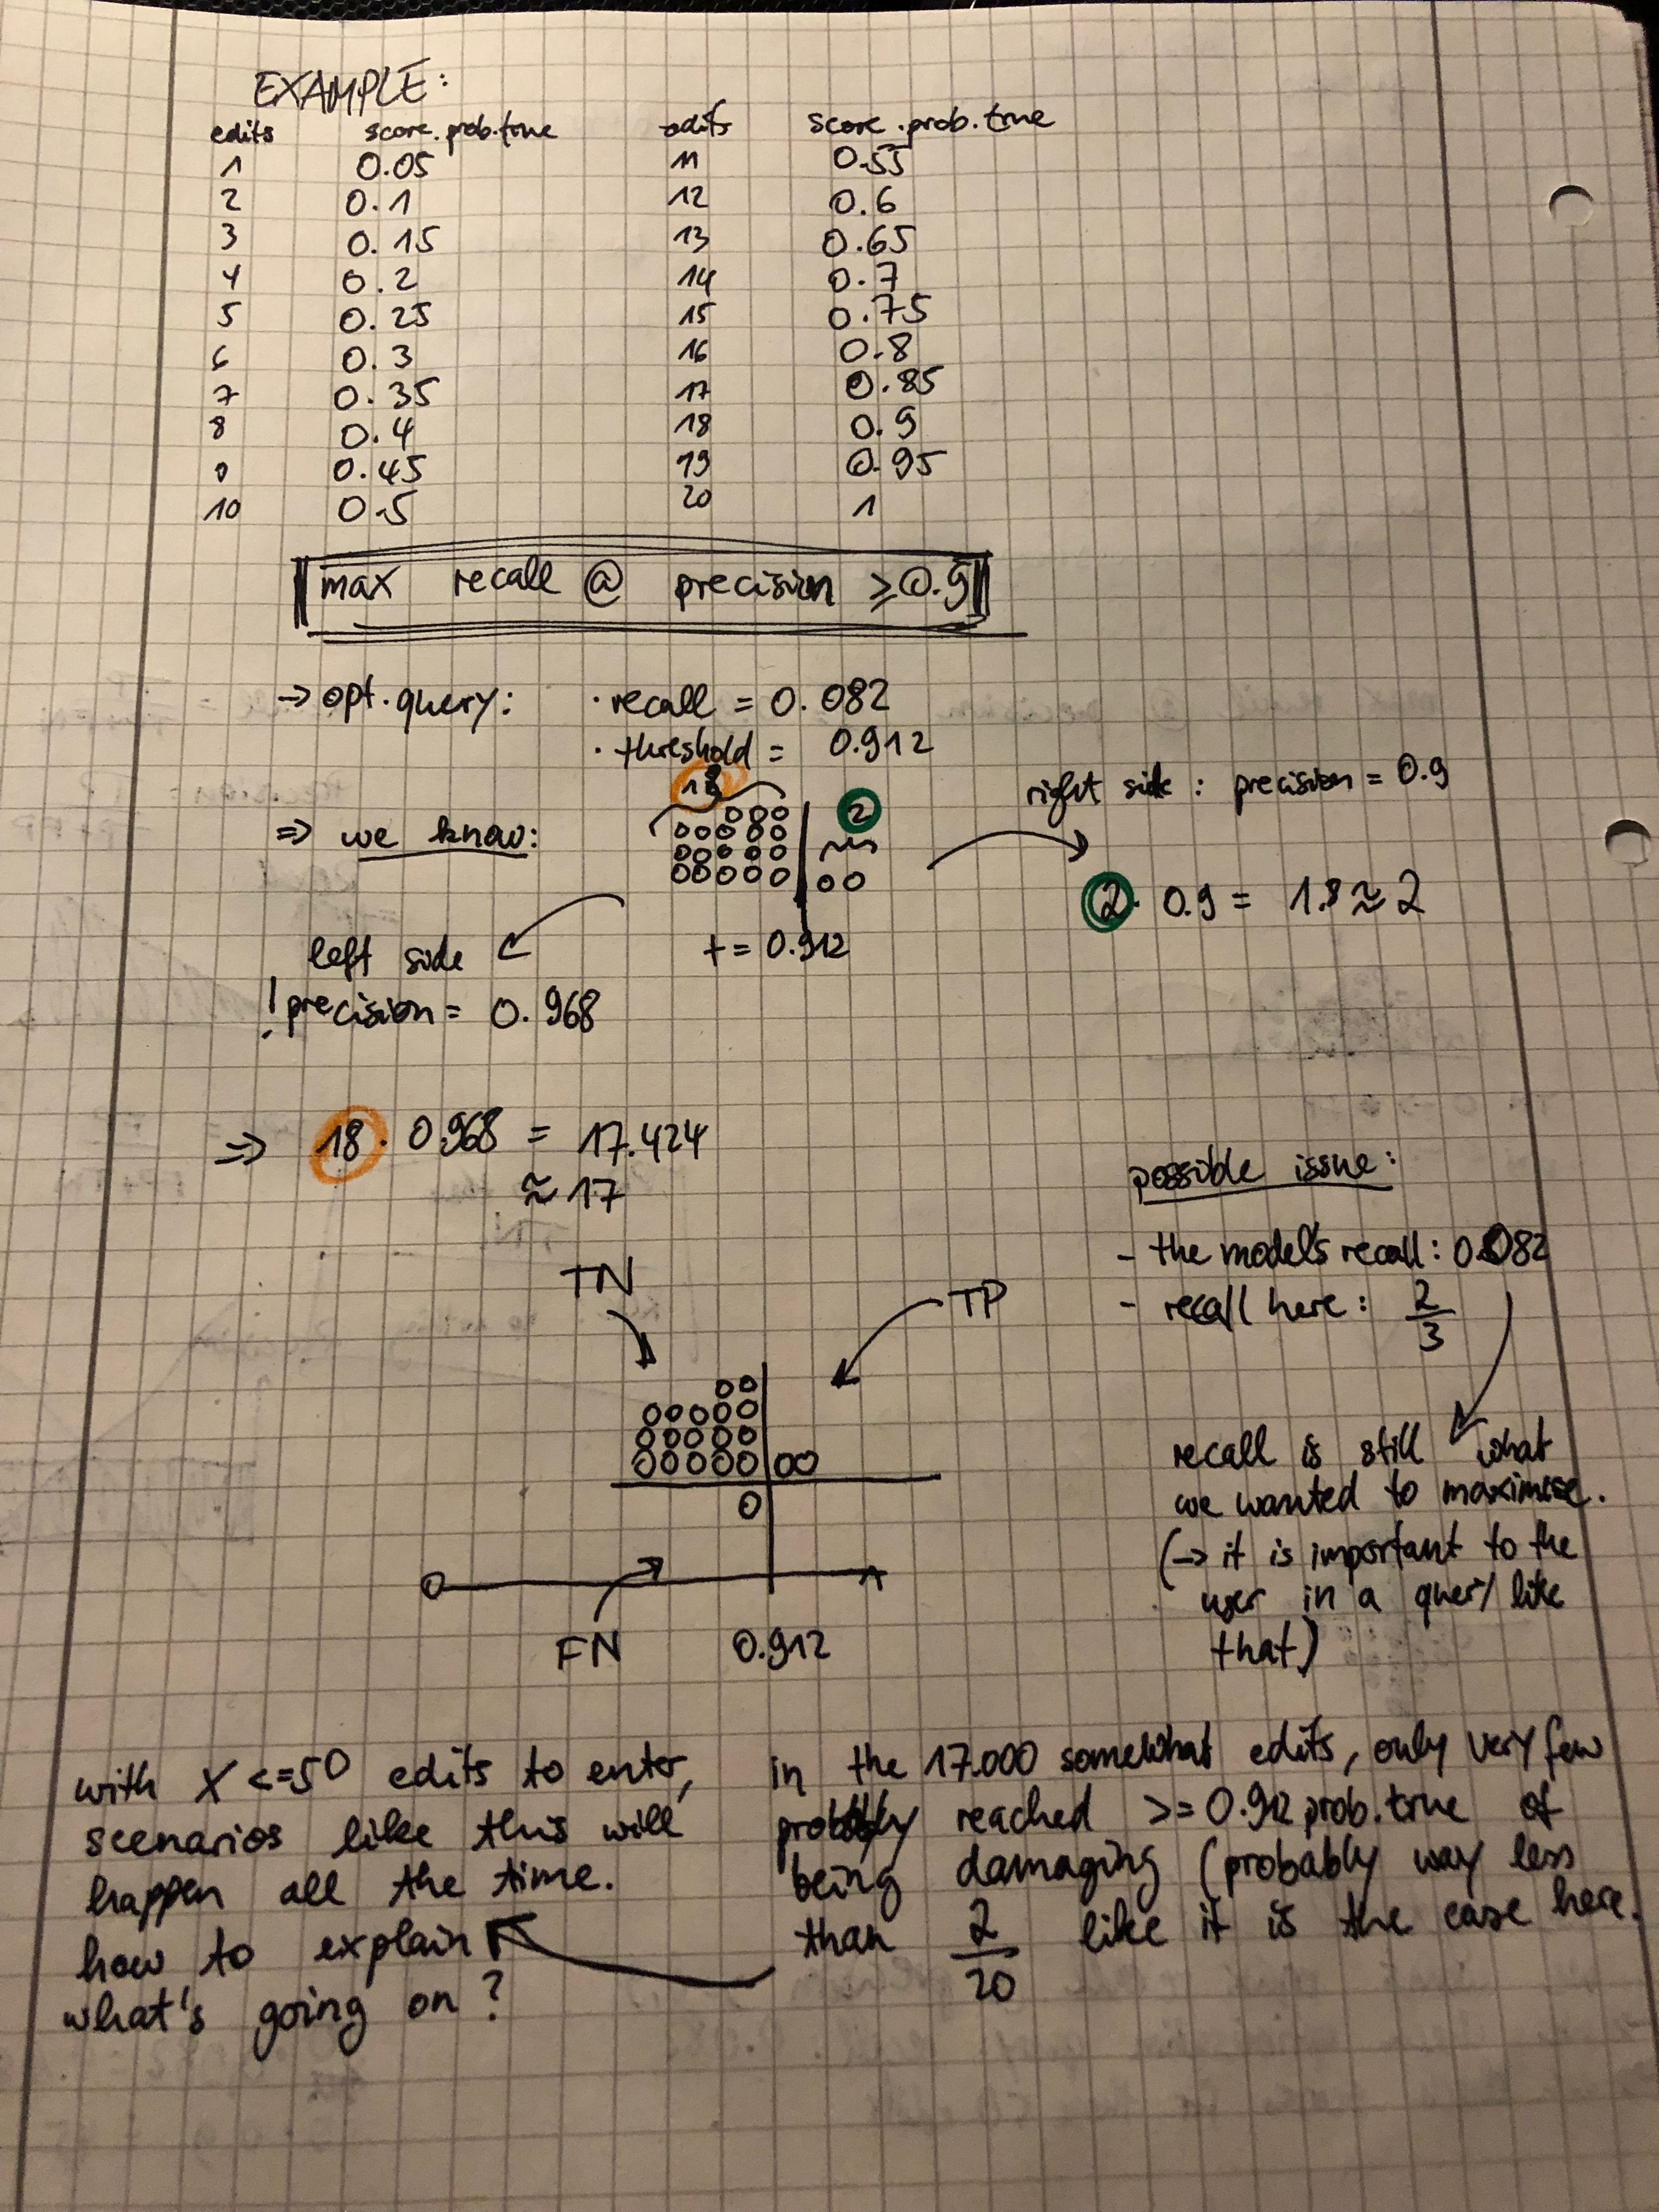
\includegraphics[scale=0.11]{resources/7/visualisationProcessExample}
\end{description}
\item \url{https://beta.observablehq.com/@mbostock/d3-histogram}
\begin{description}
\item Histogram. 
\begin{itemize}
\item Insert score.probability.true values into the array \checkmark
\item Manually paint threshold ontop of it (?)
\item Differently color bars to account for probabilities of TP/FP and TN/FN distributions (?)1
\end{itemize}
\end{description}
\item \url{https://bl.ocks.org/mbostock/4062085}
\begin{description}
\item Originally Population Pyramid
\item Same approach as for the histogram, but maybe easier to color bars (multiple colors)?
\end{description}
\end{itemize}
%
%
%
\end{document}